\chapter{Software}
    Tato kapitola se věnuje popisu návrhu softwaru pro jednotlivé části systému řízení akvária. Jak již bylo zmíněno v předchozích kapitolách, systém se skládá z řídicí jednotky, ke které jsou připojeny jednotlivé periferie a která komunikuje s webovým serverem za pomoci WiFi. Každá ze zmíněných částí pak potřebuje vlastní zdrojový kód. 
    
    K programování a testování byla použita dvě vývojová prostředí. Visual Studio Code je open source řešení spravované společností Microsoft a díky široké škále doplňků umožňuje velmi univerzální použití. S přidaným rozšířením ESP-IDF je také preferovaným prostředím společnosti Espressif, bylo tedy využito pro tvorbu kódu řidicí jednotky, stejně tak i pro webové rozhraní. Pro programování periferií pak bylo zvoleno prostředí MPLAB X. Jedná se o řešení společnosti Microchip určené speciálně pro programování mikrokontrolerů této firmy. Součástí je kromě samotného editoru také kompilátor, možnost debugování kódu nebo modul zvaný Code Configurator sloužící pro generování jednoduchého HAL (Hardware Abstraction Level) kódu.

    V této chvíli software odpovídá podobě zbytku zařízení -- tedy jedná se o prototyp určený primárně k demonstraci funkce zařízení. Aby byl kód použitelný v reálné aplikaci a choval se zde spolehlivě je potřeba podrobit jej rozsáhlejšímu testování a také lépe ošetřit chování zařízení v různých nežádoucích stavech.   

% \clearpage
\section{Architektura}
    Na obr.~\ref{fig:sw-blokove-schema} se nachází blokové schéma systému z pohledu softwaru. Obrázek slouží primárně pro lepší orientaci čtenáře v této kapitole, obsahuje pouze klíčové části a některé věci zjednodušuje. Podrobněji se jednotlivým blokům věnují další podkapitoly. Obdélník popsaný v obrázku jako \uv{Periferie} popisuje strukturu kódu platnou pro všechny periferie, je ale samozřejmé že periferií této struktury bude v systému připojeno vícero.

    Propojení přerušovanými šipkami v obrázku značí komunikaci mezi dvěma částmi s odlišným programem. Z hlediska internetové komunikace se navržené zařízení chová jako klient, tedy neposlouchá na žádném portu a z vnější sítě není nijak dostupné. Webový server disponuje datovým rozhraním (API), kterého se zařízení v pravidelných intervalech dotazuje na případné změny konfigurace a prostřednictvím kterého zasílá na server data ze svého běhu. Při komunikaci mezi řídicí jednotkou a periferiemi pak řídicí jednotka funguje jako \uv{master} a periferie odpovívají pouze v reakci na dotaz z její strany.

    % Blokove schema
    \begin{figure}[h!]
        \centering
        \begin{tikzpicture}[
            module/.style={%
        draw, rounded corners,
        minimum width=#1,
        minimum height=7mm,
        font=\sffamily,
        align=center
        },
    module/.default=2cm,
    >=LaTeX]
        
            % ridici
            \node[module] (freertos) {Free RTOS};
            \node[module, below=of freertos] (tasks) {Tasks};
            \node[module=1cm, below right=9mm and -7mm of tasks] (task1) {Relé};
            \node[module=1cm, below left= 9mm and -8mm of tasks] (task2) {WiFi};
            \node[module=1cm, below right= 3mm and 4mm of tasks] (task3) {CAN};
            \node[module=1cm, below left= 3mm and 4mm of tasks] (task4) {Status};

            \node[fit=(task1) (task2) (task3) (task4) (freertos), draw, inner sep=2mm,label={[yshift=2mm, font=\sffamily]Řídicí jednotka}] (fitridici) {};
            % Connections
            \foreach \i in {1,2,3,4}
                \draw[->] (tasks)--(task\i);
            \draw[<->] (tasks)--(freertos);

            % WS
            \node[module, below=1.5cm of {task4.west|-fitridici.south}, anchor=north west] (api) {API};
            \node[module, below=of api] (php) {PHP};
            \node[module, below=of php] (mysql) {mySQL DB};
            \node[module, right= of php] (userweb) {Uživatelský \\panel};
            \node[fit={(php) (userweb) (api) (mysql) (mysql-|fitridici.west) (mysql-|fitridici.east) }, draw, inner xsep=\pgflinewidth, inner ysep=2mm, label={[yshift=2mm, font=\sffamily]Web server}] (fitWS) {};
            \draw[<->] (api)--(php);
            \draw[<->] (php)--(mysql);
            \draw[<->] (php)--(userweb);
        
            % perif
            \node[module, right=1.5cm of {task3-|fitridici.east}] (isr) {ISR};
            \node[module, right=3mm of isr.north east, anchor=north west] (can) {Obsluha\\CAN příkazů};
            \node[module, above= 7mm of can.north east, anchor=south east] 
                (programloop) {Smyčka programu};
            \node[module, above=5mm of programloop] (dataprocess) {Zpracování dat};
            
            \node[fit={(can) (isr) (dataprocess|-fitridici.south) (dataprocess|-fitridici.north)}, draw, inner xsep=2mm, inner ysep=\pgflinewidth, label={[yshift=2mm, font=\sffamily]Periferie}] (fitperif) {};
            \node[module, right=1.5cm of dataprocess] (sensory) {Sensory};
            \draw[->] (isr)--(can);
            \draw[<->] (programloop)--(dataprocess);
            
            %arrow between boxes
            \draw[<->,dashed] (task2) to [out=-135,in=90] (api);
            \draw[->,dashed] (task3)--(isr);
            \draw[->,dashed] (can) to [out=-150,in=-45] (task3);
            \draw[<-,dashed] (dataprocess) -- (sensory);
        \end{tikzpicture}
        
        \caption{Zjednodušená architektura softwaru systému.}
        \label{fig:sw-blokove-schema}
    \end{figure}

    Jelikož jsou řídicí jednotka i periferie programovány ve stejném jazyce (C/C++), lze mezi nimi část kódu sdílet. Tímto způsobem lze částečně předejít chybám v komunikaci modulů mezi sebou. Společná část kódu obsahuje definice datových typů a konstant používaných při komunikaci po sběrnici CAN.  

\section{Popis CAN komunikace}
    Protokol CAN je poměrně rozsáhlý a velká část organizace komunikace je řešena přímo hardwarovou periferií mikrokontroleru. Pro úspěšnou a efektivní komunikaci bylo potřeba nastavit oba typy mikrokontrolerů stejně a stanovit společný standart komunikace. Systém popsaný v této práci pracuje s frekvencí \qty{125}{kHz} a používá standartní strukturu rámců s identifikátorem zprávy dlouhým 11 bitů (standart CAN 2.0B umožňuje také délku 29 bitů). Sběrnice CAN má implementovaný princip arbitrace, pokud začne komunikovat více zařízení současně, odešle se zpráva mající identifikátor s nejvyšší prioritou. Logická nula se jeví na sběrnici jako dominantní, jednička naopak jako recesivní. Pokud zařízení odesílá recesivní signál a zároveň čte ze sběrnice signál dominantní, znamená to pro něj ztrátu arbitace a přestává vysílat, jelikož na sběrnici je v danou chvíli vysílaná zpráva s vyšší prioritou. Po skončení vysílání pak přerušené zařízení pokus opakuje.
    
        \begin{figure}[h!]
            \centering
            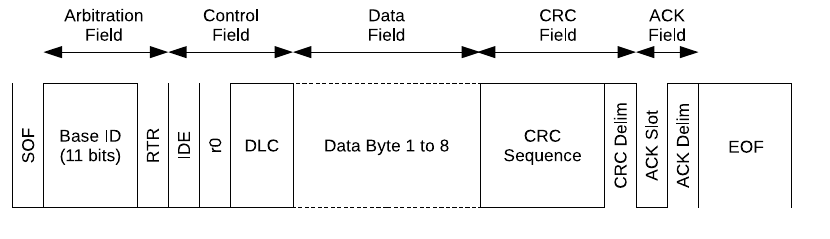
\includegraphics[width=0.8\textwidth]{obrazky/can-frame.png}
            \caption{Struktura datového rámce sběrnice CAN. Převzato z~\cite{esp32-datasheet}}
            \label{fig:obrazky/can-frame.png   }
        \end{figure}
        

    V navrženém systému nese identifikátor zprávy dvě informace. První tři odesílané bity značí typ zprávy. Rozlišena je zpráva určené všem jednotkám (BR -- Broadcast), zpráva od řídicí jednotky k periferiím (TS -- master To Slave), od periferie zpět k řídicí jednotce (TM -- slave To Master) a debug zpráva sloužící k odeslání diagnostických dat nezávisle na ostatní komunikaci. Zbylých 8 bitů pak tvoří adresu jednotky odesílají zprávu (v případě TM) resp. zprávu přijímající (v případě TS). 
    
    Adresy jednotlivých modulů by měly být po startu systému nebo připojení nové jednotky automaticky přiděleny tak, aby nedošlo ke kolizi adres ani v případě připojení několika sensorů stejného typy. Princip adresace spočívá v sérii několika BR zpráv. Po startu systému pošle řídicí jednotka požadavek na adresaci, jako odpověď odešlou jednotky periferíí své unikátní sériové číslo přičemž pouze jedna ze zpráv vyhraje arbitraci. Řídící jednotka odpoví zprávou, která obsahuje sériové číslo úspěšné jednotky a přidělenou osmibitovou adresu. Následně zopakuje požadavek adresace a odpoví již pouze jednotky bez adresy, po dokončené adresaci pak neodpoví žádná jednotka. Pokud je do běžícího systému připojena nová periferie, odešle sama BR zprávu s požadavkem na přidělení adresy.

    Ačkoliv je tento princip vymyšlen, v rámci prototypu prozatím není implementován a otestován a každý typ periferie má pevně přidělenou adresu, lze tedy připojit pouze jednu periferii stejného typu. V současné chvíli je toto řešení dostačující.



\section{Firmware řídící jednotky}
    Firma Espressif nabízí pro své mikrokontrolery dva základní frameworky. Oba jsou vyvíjeny jako open-source a jsou tedy také volně dostupní pro jakékoliv použití. Univerzálním řešením vhodným i pro komerční aplikace je ESP-IDF (Espressif Integrated Development Framework). Pro hobby projekty lze využít také Arduino framework, který je taktéž oficiálně podporovaný. Poslední novinkou je pak možnost programování v jazyce Rust namísto klasického C/C++, tento projekt je vytvářen komunitou uživatelů za podpory společnosti Espressif, prozatím ale nebyla oficiálně vydána stabilní verze. 

    \subsection{FreeRTOS}
        V rámci této práce je využit framework ESP-IDF, který obsahuje podporu pro jednoduchý operační systém Free RTOS a také drivery pro všechny hardwarové periferie mikrokontroleru~\cite{espressif-idf}.

        Systém FreeRTOS umožňuje vytvářet tzv. tasky neboli samostatné procesy které běží z pohledu uživatele paralelně. Jelikož má zvolený mikroprocesor dvě jádra, mohou dva tasky běžet skutečně paralelně, více procesů se pak ve svém běhu střídá a běží tak přerušovaně, vůči sobě pseudoparalelně. O tuto režii se stará samotný operační systém a programátor má několik možností jak tento proces ovlivnit. V případě vytížení procesoru systém přiděluje čas na základě nastavených priorit a dá přednost tasku s vyšší prioritou, může se tak stát, že některý proces zůstane pozastaven na dlouhou dobu. Při tvorbě kódu je potřeba mít toto na paměti, vhodně zvolit priority tasků a také průběžně sledovat vytížení procesoru jednotlivými tasky.  

        Aby byl kód tzv. thread-safe, tedy bezpečný pro přístup z více vláken, je potřeba ošetřit případy, kdy více tasků pracuje se stejnými daty nebo přistupuje ke stejné periferii mikrokontroleru. K tomuto účelu FreeRTOS nabízí synchronizační objekty jako jsou mutexy, semafory případně fronty. 

    \subsection{Indikace stavu zařízení}
        Šasi řídicí jednotky je vybaveno adresovatelným barevným LED páskem sestávajím ze čtyř diod jejichž úkolem je signalizovat uživateli stav zařízení. Jednotlivé stavy spolu s popisem diod jsou zobrazeny na obr.~\ref{fig:stavove-led-mainboard}. Každý task, který je součástí procesu diagnostiky má svou vlastní globální proměnnou do které ukládá svůj stav. Dvakrát za vteřinu se pak spustí jednoduchá diagnostická funkce (běží v rámci vlastního tasku), která jednotlivé stavové proměnné přečte, vyhodnotí celkový stav zařízení a aktualizuje barvu stavových LED. 
        \begin{figure}[h!]
            \centering
            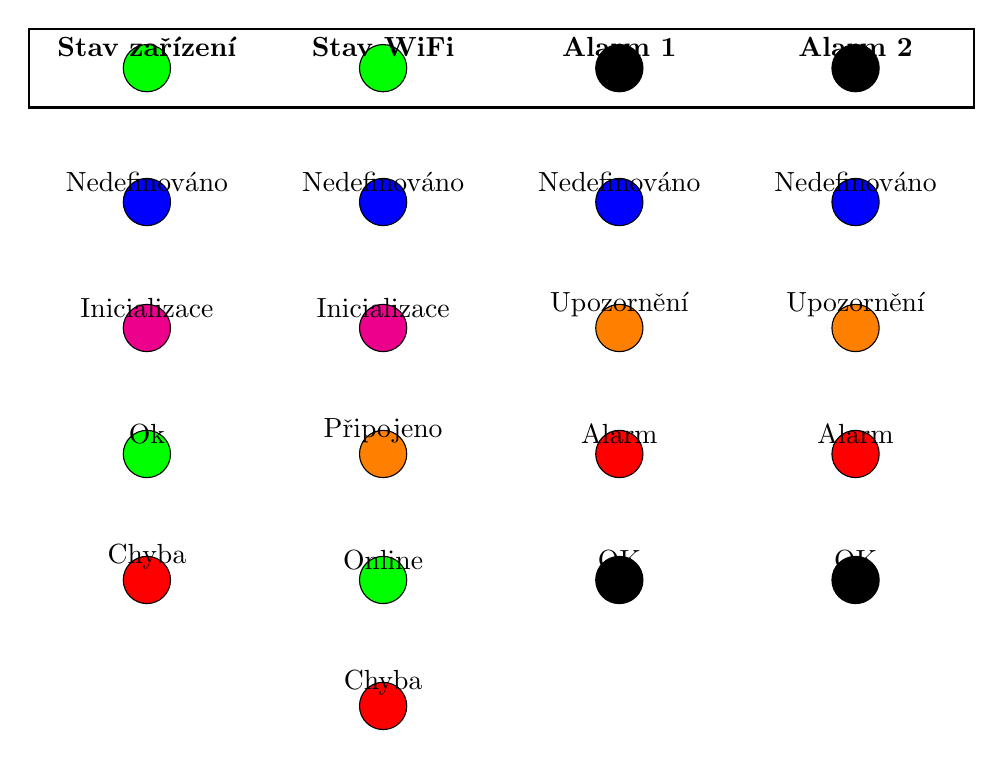
\begin{tikzpicture}
                % Draw a rectangle
                \draw[thick] (0,0) rectangle (3*4,1);
                
                % Draw and fill four colorful circles
                \filldraw[fill=green,draw=black,thin]  (3*0.5, 0.5) circle (0.3) node[align=center,above=0.5] {\textbf{Stav zařízení}};
                \filldraw[fill=green,draw=black,thin]  (3*1.5, 0.5) circle (0.3) node[align=center,above=0.5] {\textbf{Stav WiFi}};
                \filldraw[fill=black,draw=black,thin]  (3*2.5, 0.5) circle (0.3) node[align=center,above=0.5] {\textbf{Alarm 1}};
                \filldraw[fill=black,draw=black,thin]  (3*3.5, 0.5) circle (0.3) node[align=center,above=0.5] {\textbf{Alarm 2}};

                % Draw and fill four colorful circles
                \filldraw[fill=blue,draw=black,thin]    (3*0.5, -1.5*0.8) circle (0.3) node[align=center,above=0.35] {Nedefinováno};
                \filldraw[fill=blue,draw=black,thin]    (3*1.5, -1.5*0.8) circle (0.3) node[align=center,above=0.35] {Nedefinováno};
                \filldraw[fill=blue,draw=black,thin]    (3*2.5, -1.5*0.8) circle (0.3) node[align=center,above=0.35] {Nedefinováno};
                \filldraw[fill=blue,draw=black,thin]  (3*3.5, -1.5*0.8) circle (0.3) node[align=center,above=0.35] {Nedefinováno};

                % Draw and fill four colorful circles
                \filldraw[fill=magenta,draw=black,thin] (3*0.5, -3.5*0.8) circle (0.3) node[align=center,above=0.35] {Inicializace};
                \filldraw[fill=magenta,draw=black,thin] (3*1.5, -3.5*0.8) circle (0.3) node[align=center,above=0.35] {Inicializace};
                \filldraw[fill=orange,draw=black,thin]  (3*2.5, -3.5*0.8) circle (0.3) node[align=center,above=0.35] {Upozornění};
                \filldraw[fill=orange,draw=black,thin]  (3*3.5, -3.5*0.8) circle (0.3) node[align=center,above=0.35] {Upozornění};

                % Draw and fill four colorful circles
                \filldraw[fill=green,draw=black,thin]   (3*0.5, -5.5*0.8) circle (0.3) node[align=center,above=0.35] {Ok};
                \filldraw[fill=orange,draw=black,thin]  (3*1.5, -5.5*0.8) circle (0.3) node[align=center,above=0.35] {Připojeno};
                \filldraw[fill=red,draw=black,thin]   (3*2.5, -5.5*0.8) circle (0.3) node[align=center,above=0.35] {Alarm};
                \filldraw[fill=red,draw=black,thin]  (3*3.5, -5.5*0.8) circle (0.3) node[align=center,above=0.35] {Alarm};

                % Draw and fill four colorful circles
                \filldraw[fill=red,draw=black,thin]     (3*0.5, -7.5*0.8) circle (0.3) node[align=center,above=0.35] {Chyba};
                \filldraw[fill=green,draw=black,thin]   (3*1.5, -7.5*0.8) circle (0.3) node[align=center,above=0.35] {Online};
                \filldraw[fill=black,draw=black,thin]   (3*2.5, -7.5*0.8) circle (0.3) node[align=center,above=0.35] {OK};
                \filldraw[fill=black,draw=black,thin]   (3*3.5, -7.5*0.8) circle (0.3) node[align=center,above=0.35] {OK};

                % Draw and fill four colorful circles
                \filldraw[fill=red,draw=black,thin]     (3*1.5, -9.5*0.8) circle (0.3) node[align=center,above=0.35] {Chyba};
            \end{tikzpicture}
            
            \caption{Stavové LED řídicí jednotky.}
            \label{fig:stavove-led-mainboard}
        \end{figure}

    \subsection{}



\section{Firmware periferií}
\section{Webové rozhraní}
    Aby bylo možné systém konfigurovat a monitorovat bylo zapotřebí navrhnout a vytvořit webové rozhraní. Důležitým krokem v rozhodování byla volba, zda bude MCU řídicí jednotky sloužit přímo jako webový server nebo pouze jako klient. První scénář klade podstatně vyšší nároky na zatížení a paměť MCU, výhodou je ale velmi jednoduchý systém, který funguje samostetně bez nutnosti externího serveru případně také bez připojení k internetu (ESP32 může sloužit přímo jako přístupový bod). Výhodou druhé varianty je větší flexibilita, externí server má nesrovnatelně vyšší výkon a kapacitu úložiště a umožní tak tvorbu mnohem komplexnější webové stránky, která bude (v případě připojení serveru do internetu) dostupná odkudkoliv. Server zároveň může ukládat měřená data a ta tedy budou dostupná i v případě, že samotné zařízení je mimo provoz nebo není připojeno k síti.

    V rámci realizace této práce byla zvolena varianta externího serveru. Jádro vytvořené webové aplikace tvoří program v jazyce PHP, který zpracovává jak požadavky uživatele, tak i samotného zařízení. Na pozadí dále běží databázový server s otevřeným systémem MySQL sloužící k uchování provozních dat. V databázi jsou uloženy údaje o uživatelích, systémech akvárií (tedy řídicí jednotka a k ní připojené periferie) a jejich konfigurace a data získaná ze senzorů. Struktura tabulek databáze je zobrazena na obr.~\ref{TODO}. V záznamu odpovídajícímu danému systému akvária je uložen číselný údaj o aktuální verzi konfigurace. Pokud uživatel konfiguraci modifikuje, toto číslo se inkrementuje na což následně zareaguje zařízení a vyžádá si ze serveru novou verzi konfigurace. 

    Zařízení komunikuje s webem pomocí aplikačního rozhraní (API), které tvoří nenáročný způsob komunikace využívající formát JSON. Jednotlivé adresy API rozhraní jsou přehledně popsány v tab.~\ref{TODO}. 

